% !TEX encoding = IsoLatin 

% Affinch� gli accenti vengano accettati, assicurati che la codifica di questo file
% sia ISO 8859-1

% PER OTTENERE IL PDF, digitare da terminale
% ./makepdfplease
% 
\chapter[Valutazione dei risultati][]{5. Valutazione dei risultati}

Dopo l'implementazione dei due prototipi, possiamo introdurre la loro valutazione con l'uso della classe Scorer della libreria SpaCy.
La terminologia Scorer proviene dal mondo del Machine Learning ed indica l'affidabilit� della predizione di una data entit� in termini di \textbf{precision}, \textbf{recall} e \textbf{accuracy}.

\section{Scorer Class}
Lo Scorer � la classe fornita da SpaCy per valutare le performance di un modello annotatore per ogni singola entit� basandosi sulle 
annotazioni prodotte da tale modello.
Lo Scorer richiede all'utente della libreria di avere a disposizione l'output del modello annotatore e le gold annotations della Ground Truth.
Per ogni annotazione si crea un oggetto spacy.Span e si crea una lista di Span, che chiameremo labelled\_entities\_span\_list; si potr� poi utilizzare la lista di gold annotations per creare il relativo \textbf{item} che descrive l'annotazione di un documento:

\begin{lstlisting}[language=Python, caption=Esempio di item]
item = Example.from_dict(labelled_entities_span_list, 
                         {"entities": [[start_offset, end_offset, word]
                                      for [start_offset, end_offset, word]
                                      in gold_annots]})
\end{lstlisting}

Si crea un Example per ogni documento annotato e si pongono gli item in una \textbf{item\_list}.
Tutti i dati annotati dal modello annotatore sono ora nella item list ed � dunque possibile invocare 
il task di score vero e proprio:
\begin{lstlisting}[language=Python]
    scores = scorer.score(item_list)
\end{lstlisting}

\section{Confronto tra i due approcci}
Nella tabella scores-comparisons.pdf riporta i valori di Precision, Recall e Accuracy ottenuti per ogni entit� contemplata nel task di 
classificazione.


%allora\includegraphics[width=16cm, height=30cm,page=1]{scores-comparisons.pdf} %width=, height=, page=,
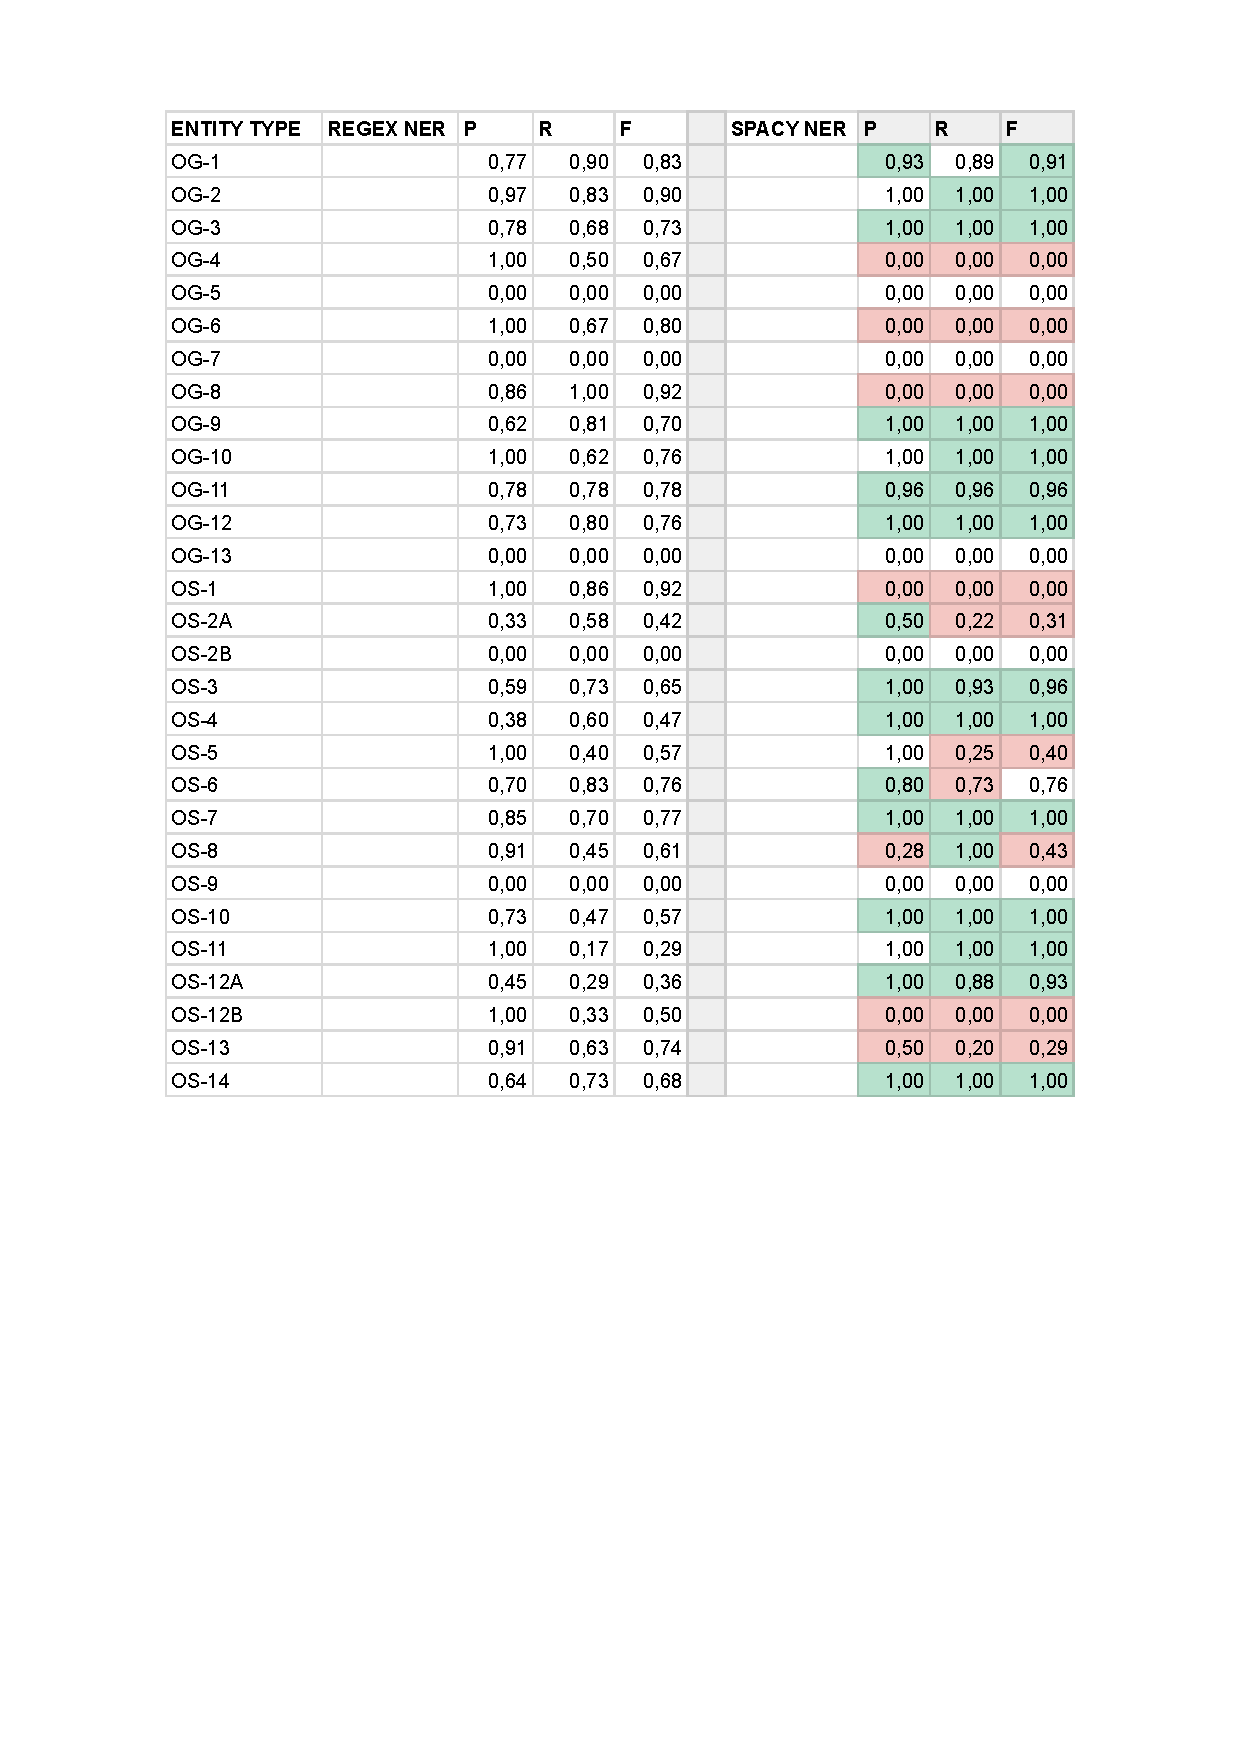
\includegraphics[trim=0 300 0 0, clip, width=\textwidth,height=\textheight,keepaspectratio, page=1]{confronti.pdf} 
\captionof{figure}{confronto tra l'approccio regex(sinistra) e NN(destra)}
Si pu� facilmente notare come molte entit� di tipo \textbf{Categoria} vedono valori di precision recall e accuracy migliori nell'approccio Machine Learning; questo miglioramento si rivela significativo in circa il 60\% delle entit� categoria.
Nel restante 40\% delle categorie si registra un peggioramento delle performance del Machine Learning, che in pochi ma significativi casi abbatte a zero le score.
Questo pu� essere dovuto alla mancanza di esempi numerosi per tutte le entit�: 
ci� porterebbe il modello a funzionare molto bene nel riconoscere le entit� ben rappresentate dalla ground truth,
ma anche a funzionare peggio per tutte le entit� meno note.
Le regex invece, fornendo a priori i pattern di ogni entit�, non soffrono della mancanza di esempi. 

Come sottolineato precedentemente, l'approccio NER con regex non ha grandi margini di miglioramento dell'accuratezza:
in sintesi � un approccio rigido, che in caso di inclusione di nuovi pattern testuali 
richiederebbe la continua modifica di una regex in forme sempre pi� complesse, risolvendosi in
problemi di manutenzione, di testing, di leggibilit� e talvolta di sicurezza.
Nel caso del Machine Learning un task di \acrfull{named-entity-recognition} pu� avere risultati migliori delle regex, 
ma pu� soffrire di carenza di esempi per alcune entit�.
Su questa base si potrebbe proporre l'uso combinato degli output di entrambi i modelli: in particolare,
si potrebbe ricorrere al modello regex per le entit� meno assimilate dal modello \acrfull{machine-learning}
, preferendo invece quest'ultimo
per le entit� su cui gli score descrivono prestazioni migliori.



\section{Human In The Loop}
Fin qui il lavoro di \acrshort{societa-soa} extraction ci ha portati a considerare due tecnologie molto diverse per
approccio e manutenibilit�.

In particolare, le \textbf{regex} risultano di risultato immediato poich� in pochi minuti ci consentono di
svolgere un'estrazione di dati SOA con discreti valori di recall,
ma soffrono di \textbf{scarsa leggibilit�}, manutenzione problematica e decisamente \textbf{error-prone} ;
nonostante un incoraggiante risultato immediato, non permettono di migliorare in maniera efficiente l'estrazione di 
entit� per tutta una serie di fattori.
Consideriamo ad esempio il manutentore a cui toccher� estendere la regex in produzione \(reg\_prod\sb{n}\); 
il suo compito sar� tipicamente quello di trasformare la \(reg\sb{prod}\) in una \(reg\_prod\sb{n+1}\)
in maniera da includere i nuovi pattern \( p\sb{m+1} , \ldots , p\sb{m+k} \).
Le domande che ci poniamo sono allora le seguenti:
Quella vecchia regex \(reg\_prod\sb{n}\) sar� stata fino ad allora documentata per tenere traccia dei
pattern precedenti \( p\sb{1}, \ldots ,  p\sb{m} \) ?
Oppure spetter� al programmatore ricordare tutti i singoli pattern che venivano catturati con la precedente versione della regex?
E la regex avr� dei dati di \textbf{testing}, per verificare che la nuova versione \(reg\_prod\sb{n+1}\)
non comprometta i pattern fino ad allora accettati?
Tutte queste domande si ritrovano nell'indagine statistica di \say{Regexes are hard} \cite{RegexesAreHard}, 
dove la risposta � negativa: le regex vengono usate perlopi� senza documentazione e senza dati di test,
per cui un sistema basato su sole regex � nel tempo inefficiente nel miglioramento della \acrlong{Precision}.

Al contrario, le reti neurali possono nel tempo \say{imparare meglio} le entit� con cui hanno a che fare ma richiedono un consistente lavoro umano di annotazione e classificazione delle entit� presenti nei dati stessi;
in altre parole, mancano dell'immediatezza delle regex ma rendono fattibile il \textbf{fine-tuning} del sistema classificatore.

%\includegraphics[trim=0 300 0 0, clip, width=\textwidth,height=\textheight,keepaspectratio, page=1]{grafo_regex.pdf}
%\includegraphics[trim=0 300 0 0, clip, width=\textwidth,height=\textheight,keepaspectratio, page=1]{grafo_nn.pdf}
%\includegraphics[trim=0 300 0 0, clip, width=\textwidth,height=\textheight,keepaspectratio, page=1]{grafo_regexnn.pdf} 

I rispettivi punti di forza e di debolezza delle due metodologie risultano complementari, per cui ha senso combinarli in un
unico sistema che sfrutti i vantaggi di entrambe, mitigandone gli svantaggi.

% HIL DIAGRAM
\includegraphics[trim= 10 200 0 100, clip, width=\textwidth,height=\textheight,keepaspectratio, page=1]{flow_chart_hil.pdf} 
\caption{Human In The Loop framework} 
\begin{comment}

	\begin{figure}[ht] % placed here or on the top of page
		\begin{tikzpicture}[node distance=3cm]
		%\begin{tikzpicture}%[->,shorten >=1pt,auto,node distance=2.8cm,semithick]
			\node (data) [state] {Data};
			\node (module0) [process, below=1cm of data] {regex\_ner};
			\draw [arrow] (data) -- (module0);
			\node (wl) 		[state, below=1cm of module0] {wl};
			\draw [arrow] (module0) -- (wl);
			\node (humcorr) [process, below=1cm of wl] {human\_correc};
			\draw [arrow] (wl) -- (humcorr);
			\node (l) 		[state, left of=humcorr] {labels};
			\draw [arrow] (humcorr) -- (l);
			\node (train) 	[process, below of=l] {training};
			\draw [arrow] (l) -- (train);
			\node (nn) 		[state, below of=train] {nn};
			\draw [arrow] (train) -- (nn);
			\node (module) [process, right of=nn] {nn\_usage};
			\draw [arrow] (nn) -- (module);
			\node (entities) [state, below of=module] {Entities};
			\node (entitiescorr) [state, above of=module] {Entities};
			\draw [arrow] (module) -- (entities);
			\draw [arrow] (module) -- (entitiescorr);
			\draw [arrow] (entitiescorr) -- (humcorr);
			
\begin{pgfonlayer}{background}
\filldraw [fill=black!30,draw=red] (3,-5) rectangle (-5,-13.5);
%\filldraw [fill=black!30,draw=red] (nn.south -| nn.west) rectangle (humcorr.north -| entitiescorr.east);
\end{pgfonlayer}
		\end{tikzpicture}
		\caption{Human In The Loop framework} % caption
		%\label{fig:diagram}             % for referencing of figure, key select as you wish
	\end{figure}
\end{comment}



Possiamo dunque configurare l'uso delle componenti regex, \acrshort{machine-learning}, task di creazione regex e task di 
annotazione manuale come un sistema di tipo \acrshort{human-in-the-loop}.
In tale sistema l'essere umano pi� essere utilizzato come programmatore di regex e come annotatore a pi� riprese successive.
Partendo dallo studio \say{How to invest my time} \cite{HowToInvestMyTime}, l'indicazione che traiamo per usare al meglio
il lavoro umano � investire pochi minuti sulla creazione di regex ad alta \acrlong{Recall} per poi far seguire a questa  la correzione umana delle annotazioni prodotte dalla regex stessa.
Seguendo la convenzione dello studio citato, chiameremo \say{weak labelling} l'estrazione svolta con la regex, che indicheremo con \(RE\sb{WL}\).
La \textbf{human annotation} prender� in input le \textbf{weak labels} prodotte con la  \(RE\sb{WL}\)
e produrr� annotazioni che potremo considerare  affidabili perch� verificate da un umano;
tali annotazioni costituiranno il training set della rete neurale.




